% !TEX root = ../main.tex




\chapter{The Segmental Synthesizer}\label{chap:segmental-synthesizer}

In the first stages of my implementation, synthetic contours produced were simply transplanted onto the original signals by means of pitch manipulation in Praat.
As this approach results in inconsistent quality across signals, a vocoder was used to synthesize the signals from scratch.

Even though vocoders can theoretically separate the periodic information (i.e., the \ac{F0} contour) from spectral features and aperiodicity, in reality most vocoders (in particular those based on the source-filter model) do not achieve perfect decorrelation.

This means that each set of features cannot be modeled independently of each other without significant signal degradation.
In order to model \ac{F0} independently, the generation of aperiodic and spectral features must be conditioned on the periodic features.

This was achieved in my implementation by a neural network model that takes a linguistic specification along with duration and \ac{F0} information as input, and predicts the remaining acoustic features as output.
By conditioning the training of the acoustic features not only on duration and linguistic features, but crucially also on the \ac{F0}, we are able to model the residual correlations left over by the vocoding process.
The segmental synthesizer provides a way of inhibiting the effects of the spectrum, thus making the synthesis of spectral features consistent across many possible \ac{F0} contours.

\vfill

\section{General Overview}

The pipeline of the segmental synthesizer (shown here as \autoref{fig:seg-pipeline}) is organized into two major components: a \ac{DNN} component (the blue and the green boxes) and a waveform generation component (the red box).
The \ac{DNN} component is composed of two major components: a frame prediction component (the blue box) and smoothing component (the green box).

\begin{figure}[h]
    \centering
    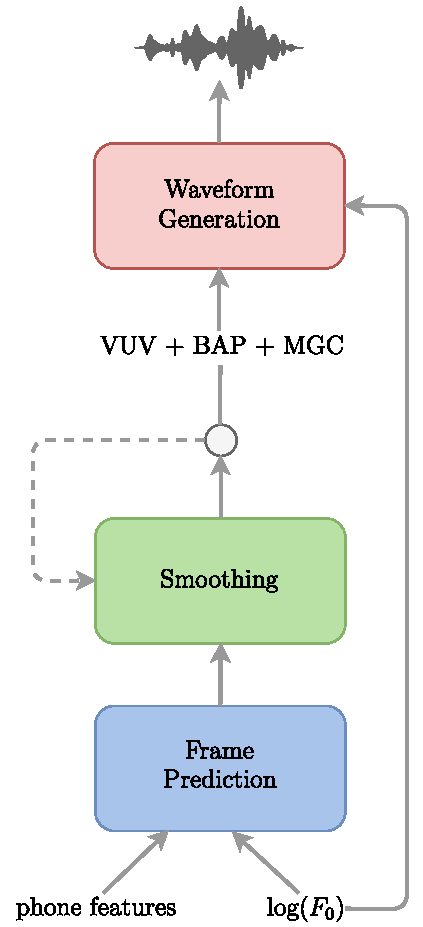
\includegraphics[scale=0.8]{figures/seg-pipeline.pdf}
    \vspace*{5mm}
    \caption[Segmental synthesizer pipeline]{Pipeline of the segmental synthesizer. The Frame Prediction component (the blue box) is a 10-layer \ac{FFNN}. The Smoothing component (the green box) is a single-layer \ac{RNN}. The Waveform Generation component (the red box) is a vocoder.}
    \label{fig:seg-pipeline}
\end{figure}

The segmental synthesizer takes a linguistic representation (i.e., phone features) and log(\ac{F0}) as input.
This information is fed to a \ac{FFNN} to predict a frame at each time step.

In order to ensure that the transitions between the frame are smooth, the output of the \ac{FFNN} is passed through an \ac{RNN}.

The output of this component, as well as the \ac{F0}, are used by a vocoder to generate a waveform.




\section{Description of the Input}

According to common practice, input frames are produced at 5~ms intervals.
The features contained in each frame consist of 225 binary features and 3 numerical features (for more details, see \autoref{chap:appendix-c}).

The binary features, which constitute the linguistic specification, are used to encode quinphone identity, i.e., information about the current phone, the previous one, the next one, the one before the previous one, and the one after the next one.
The phone set is based on the \ac{OALD} provided with Festival\footnote{\url{http://www.cstr.ed.ac.uk/projects/festival/}}, augmented with an extra symbol for silence.

The numerical features comprise: a percentage value to encode positional information within the syllable, phone duration encoded as number of frames divided by 100 to make it fit approximately within a 0--1 range, and finally, log_2(\ac{F0}) divided by 10 to make it fit approximately within a 0--1 range.
During training, the \ac{F0} information is extracted by the WORLD vocoder and linearly interpolated.

Input vectors generated by the concatenation of the binary and numerical features are normalized to a standard normal distribution.


\section{Description of the Output}

For each input frame a corresponding output frame containing acoustic features is constructed.
The output features contained in each frame consist of 2 binary features and 67 numerical features (for more details, see \autoref{chap:appendix-c}).

The binary features encode \ac{VUV} information.
The aperiodic and spectral information is extracted by the WORLD vocoder and then converted into 5 \ac{BAP} and 60 \ac{MGC} coefficients, including the corresponding gain, using \ac{SPTK}.\footnote{\url{http://sp-tk.sourceforge.net/}}
The binary and numerical information is concatenated into a single vector and then normalized to a standard normal distribution.


\section{Description of the DNN Model}

The neural network model is organized into two major components.
The first component (shown as the blue box in \autoref{fig:seg-pipeline}) is comprised of 10 feed-forward layers, each containing 1024 hidden units.
These layers are tasked with the processing of frames within each time step.

For this first component, a special type of self-normalizing feed-forward layers are used.
In \acp{SNN}, the provided activation function is modified slightly so that neuron activations will automatically converge towards zero mean and unit variance.
\acp{SNN} have been shown to outperform traditional \acp{FFNN} \citep{Klambauer2017Self}.
In my implementation, the self-normalizing modification is applied to the ELU activation function \citep{Clevert2015Fast}.

The second component (shown as the green box in \autoref{fig:seg-pipeline}) is a single forward \ac{GRU} recurrent layer with 1024 hidden units and ELU activations.
The main purpose of this component is to replace the smoothing function of the static values across frames traditionally achieved through the use of the dynamics.

The network was trained using the sum-of-squares error function, which was minimized using \ac{SGD} with Nesterov Momentum.

\section{Wave Generation}

During inference, input vectors are constructed with a synthetic \ac{F0} contour.

The input vectors are passed through the network to generate \ac{VUV}, \ac{BAP}, and \ac{MGC} coefficients.
\ac{VUV} information is used to set the unvoiced parts of the \ac{F0} contour to zero.
\ac{BAP} and \ac{MGC} coefficients are converted back to aperiodic and spectral information.

The \ac{F0} contour, the aperiodic, and the spectral information are fed to the waveform component of the pipeline (shown as the red box in \autoref{fig:seg-pipeline}) to produce an acoustic signal by means of the WORLD vocoder\footnote{\url{https://github.com/mmorise/World}}.
